\section{User Interface}
\subsection{Character User Interface}
The first iteration for the user interface is a simple CUI (Character User Interface) which directly shows the data which is gathered from the sensors and sent through the wireless connection. Because of the fact that Matlab, the chosen framework for user interface, contains an inherent CUI, there was no need to create a custom CUI. Because of this, the implementation of the CUI consisted of creating a receiver for the sensor data and transforming this data in a readable format. 

\begin{figure}[H]
	\centering
	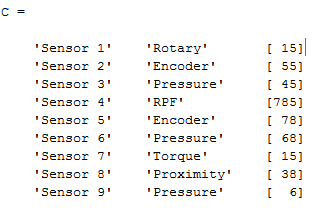
\includegraphics[width=.75\textwidth]{images/CUI}
	\caption{A sample of the CUI} 
	\label{fig:CUIV1}
\end{figure} 

\subsection{Graphical User Interface}
The first version of the GUI (Graphical User Interface) 
\begin{figure}[H]
	\centering
	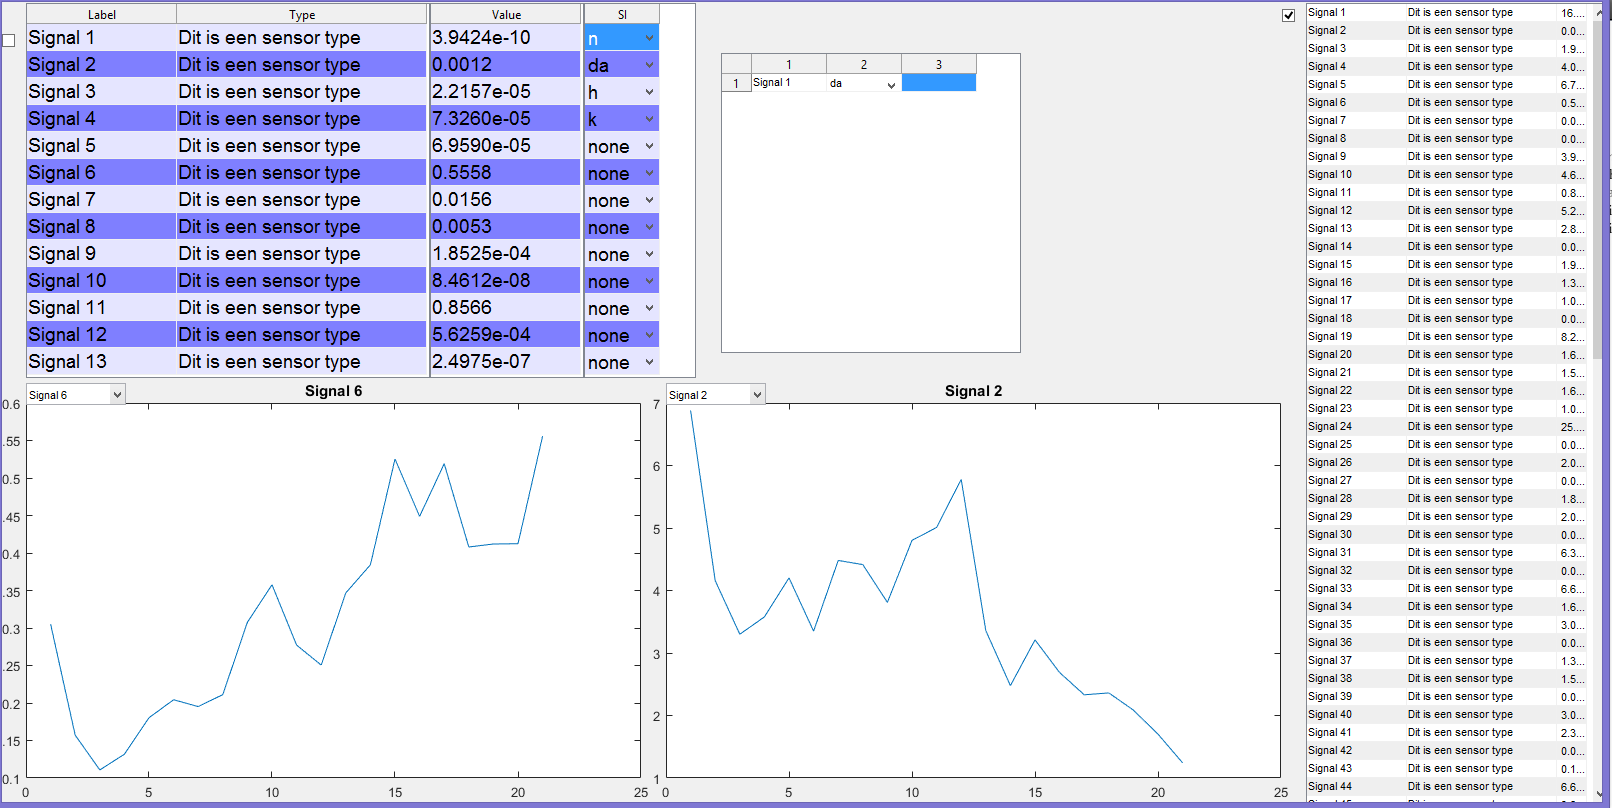
\includegraphics[width=.75\textwidth]{images/GUIV1}
	\caption{A sample of the GUI at the end of the first sprint} 
	\label{fig:GUIV1}
\end{figure} 